% ----------------------------------------------------------------------------------------------------- %
% Manual da Classe UFTeX
% 
% Versão 1.1:   Março 2016
%
% Criado por:   Tiago da Silva Almeida
% Revisado por: Tiago da Silva Almeida
%               Rafael Lima de Carvalho
%               Ary Henrique Morais de Oliveira
%
% http://uftex.sourceforge.net
% ----------------------------------------------------------------------------------------------------- %

\documentclass[tcc2]{uftex}
% ---- Esse comando cria o nome uftex estilizado
\newcommand\uftex{UF\TeX}

\usepackage{lipsum}

\usepackage[alf]{abntex2cite}
\renewcommand{\backrefpagesname}{}
\renewcommand{\backref}{}
\renewcommand*{\backrefalt}[4]{}
% ----  Esse comandos são necessário no pré-ambulo para a impressão da lista de lista abreviatuas e de símbolos
\makelosymbols
\makeloabbreviations
% ---- Início do documento
\begin{document}
  % ---- Descrição do título do trabalho 
  \title{Titulo do trabalho}
  % ---- Nome do autor ou autores do trabalho
  \author{Autor}{Sobrenome}
  \author{Autor}{Sobrenome 2}
  \class{Sistemas Digitais}
  % ---- Nome do orientador do trabalho. O último campo representa o título do professor
  \advisor{Prof.}{Tiago}{da Silva Almeida}{M.Sc.}

  \examiner{Prof.}{Dr.}{Nome do Primeiro Examinador Sobrenome}
  \examiner{Prof.}{Dr.}{Nome do Segundo Examinador Sobrenome}
  \examiner{Prof.}{Dr.}{Nome do Terceiro Examinador Sobrenome}
  % ---- Departamento representa o curso ao qual o trabalho está sendo apresentado. Descrito por meio de duas iniciais do curso
  \department{CC}
  % ---- Data da apresentação do trabalho
  \date{25}{03}{2016}
  % ---- Palavras-chaves em português do trabalho
  \keyword{\LaTeX}
  \keyword{\uftex}
  \keyword{Trabalho de Conclusão de Curso}
  \keyword{Redação Científica}
  \keyword{Extensão Universitária}
  % ---- Palavras-chaves em inglês do trabalho
  \foreignkeyword{\LaTeX}
  \foreignkeyword{\uftex}
  \foreignkeyword{Bachelor Thesis}
  \foreignkeyword{Scientific Writing}
  \foreignkeyword{University Extension}
  % ---- Comando responsável por criar a capa do trabalho e/ou folha de resto conforme a configuração exigida
  \maketitle

  \frontmatter

  % ----------------------------------------------------------------------------------------------------- %
  %  Este trecho deve ser inserido somente no caso do TCC2 já na versão FINAL
  % ----------------------------------------------------------------------------------------------------- %
  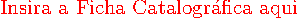
\includepdf{ficha_catalografica}
  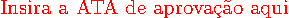
\includepdf{ata_de_aprovacao}
  % ----------------------------------------------------------------------------------------------------- %
  \dedication{A algu\'em cujo valor \'e digno desta dedicat\'oria.}

  \begin{acknowledgement}
  Gostaria de agradecer a todos.
  \end{acknowledgement}

  \begin{abstract}
  \lipsum[1]
  \end{abstract}

  \begin{foreignabstract}
  \lipsum[9]
  \end{foreignabstract}
  \printlosymbols  
  \printloabbreviations
  % ---- Cria a lista de figuras. OPCIONAL
  \listoffigures
  % ---- Cria a lista de tabelas. OPCIONAL
  \listoftables 
  % ---- Cria o sumário. OBRIGATÓRIO
  \tableofcontents % sumário
% --- Marca o inicio dos elementos textuais. Capítulos.
\mainmatter
% ---- Defino o espaçamento de um e meio centímetros
\onehalfspacing
% ----------------------------------------------------------------------------------------------------- %
% Capítulos do trabalho
% ----------------------------------------------------------------------------------------------------- %
\ChapterStart{first}{First chapter}
\chapter{Introdução}
\label{sec:introducao}
% ALTERAR texto desta seção
\noindent 
\lipsum[1]

\lipsum[2]

\lipsum[3]

\section{Licença}
\label{sec:Licenca}

\noindent 
\lipsum[4]

\lipsum[5]

\lipsum[6]

\backmatter 
\singlespacing   
% ----------------------------------------------------------------------------------------------------- %
\bibliography{manual_uftex}

\appendix
\onehalfspacing

\chapter{Sequências}
\label{ape:sequencias}

\noindent 
\lipsum[7]


\end{document}
